\documentclass{standalone}
\usepackage{tikz}
\usetikzlibrary{patterns, positioning}

\begin{document}
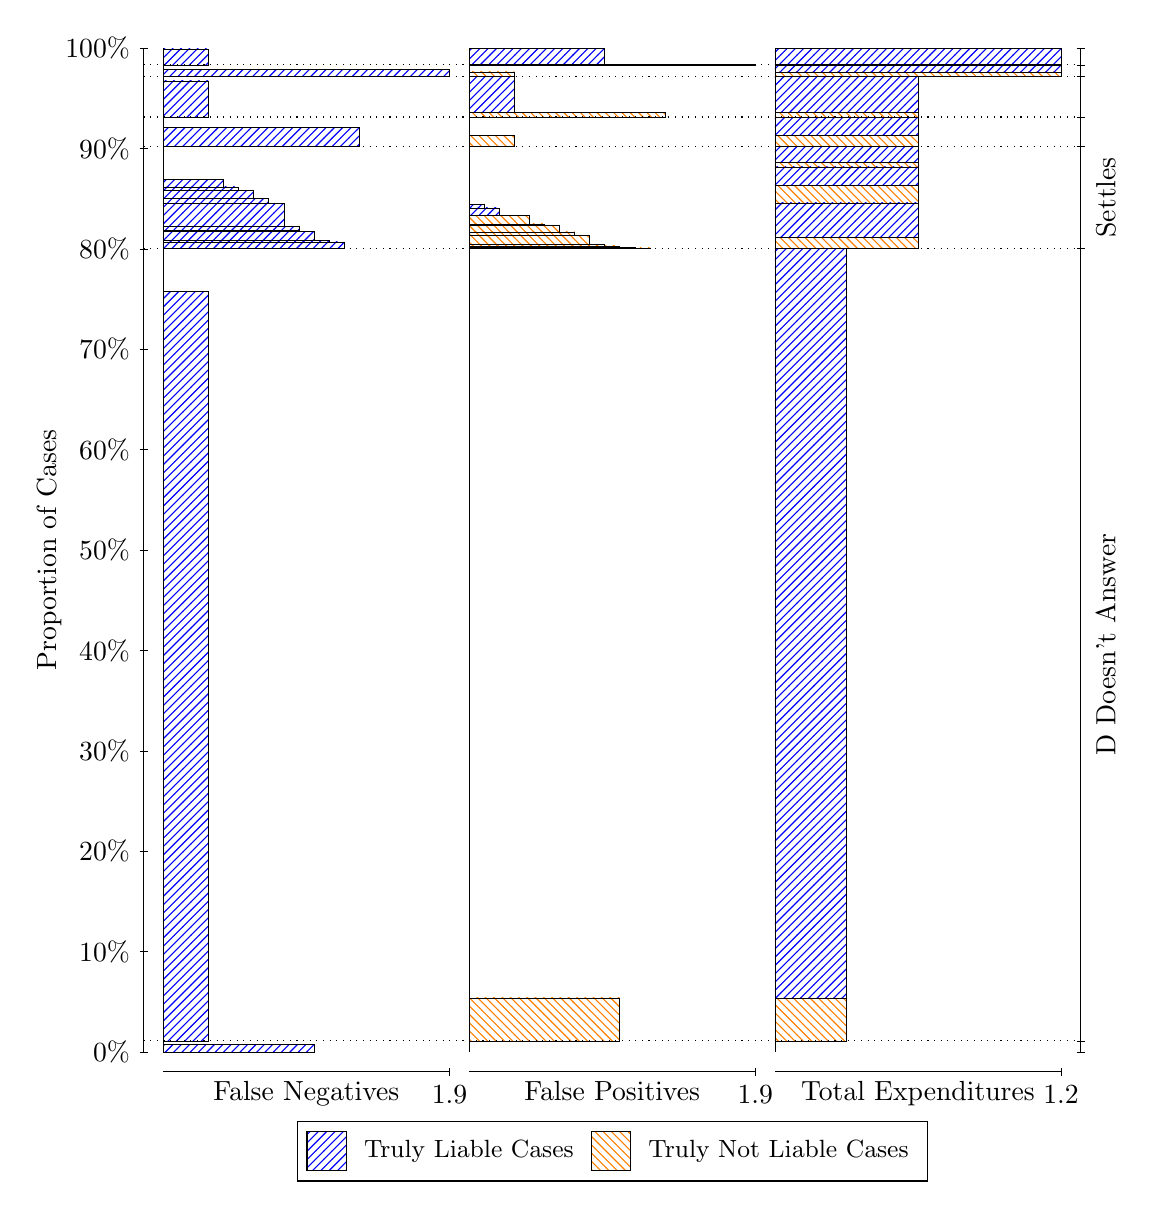
\begin{tikzpicture}
\draw[black, very thin] (1.5,1.75) -- (1.5,14.5);
\node[rotate=90, anchor=center] at (0.3, 8.125) {Proportion of Cases};
\draw[black, very thin] (1.45,1.75) -- (1.55,1.75);
\node[anchor=east] at (1.45, 1.75) {0\%};
\draw[black, very thin] (1.45,3.025) -- (1.55,3.025);
\node[anchor=east] at (1.45, 3.025) {10\%};
\draw[black, very thin] (1.45,4.3) -- (1.55,4.3);
\node[anchor=east] at (1.45, 4.3) {20\%};
\draw[black, very thin] (1.45,5.575) -- (1.55,5.575);
\node[anchor=east] at (1.45, 5.575) {30\%};
\draw[black, very thin] (1.45,6.85) -- (1.55,6.85);
\node[anchor=east] at (1.45, 6.85) {40\%};
\draw[black, very thin] (1.45,8.125) -- (1.55,8.125);
\node[anchor=east] at (1.45, 8.125) {50\%};
\draw[black, very thin] (1.45,9.4) -- (1.55,9.4);
\node[anchor=east] at (1.45, 9.4) {60\%};
\draw[black, very thin] (1.45,10.675) -- (1.55,10.675);
\node[anchor=east] at (1.45, 10.675) {70\%};
\draw[black, very thin] (1.45,11.95) -- (1.55,11.95);
\node[anchor=east] at (1.45, 11.95) {80\%};
\draw[black, very thin] (1.45,13.225) -- (1.55,13.225);
\node[anchor=east] at (1.45, 13.225) {90\%};
\draw[black, very thin] (1.45,14.5) -- (1.55,14.5);
\node[anchor=east] at (1.45, 14.5) {100\%};

\draw[black, very thin] (13.4,1.75) -- (13.4,14.5);
\draw[black, very thin] (13.35,1.75) -- (13.45,1.75);
\node[anchor=west] at (13.35, 1.75) {};
\draw[black, very thin] (13.35,1.8916) -- (13.45,1.8916);
\node[anchor=west] at (13.35, 1.8916) {};
\draw[black, very thin] (13.35,11.955) -- (13.45,11.955);
\node[anchor=west] at (13.35, 11.955) {};
\draw[black, very thin] (13.35,13.252) -- (13.45,13.252);
\node[anchor=west] at (13.35, 13.252) {};
\draw[black, very thin] (13.35,13.624) -- (13.45,13.624);
\node[anchor=west] at (13.35, 13.624) {};
\draw[black, very thin] (13.35,14.141) -- (13.45,14.141);
\node[anchor=west] at (13.35, 14.141) {};
\draw[black, very thin] (13.35,14.286) -- (13.45,14.286);
\node[anchor=west] at (13.35, 14.286) {};
\draw[black, very thin] (13.35,14.5) -- (13.45,14.5);
\node[anchor=west] at (13.35, 14.5) {};

\draw[black, very thin, pattern color=blue, pattern=north east lines] (1.75,1.75) rectangle (3.6623,1.8423);
\draw[black, very thin, pattern color=orange, pattern=north west lines] (1.75,1.8423) rectangle (1.75,1.8916);
\draw[black, very thin, pattern color=blue, pattern=north east lines] (1.75,1.8916) rectangle (2.3237,11.411);
\draw[black, very thin, pattern color=orange, pattern=north west lines] (1.75,11.411) rectangle (1.75,11.955);
\draw[black, very thin, pattern color=blue, pattern=north east lines] (1.75,11.955) rectangle (4.0447,12.038);
\draw[black, very thin, pattern color=blue, pattern=north east lines] (1.75,12.038) rectangle (3.8535,12.057);
\draw[black, very thin, pattern color=blue, pattern=north east lines] (1.75,12.057) rectangle (3.6623,12.167);
\draw[black, very thin, pattern color=blue, pattern=north east lines] (1.75,12.167) rectangle (3.4711,12.187);
\draw[black, very thin, pattern color=blue, pattern=north east lines] (1.75,12.187) rectangle (3.4711,12.233);
\draw[black, very thin, pattern color=blue, pattern=north east lines] (1.75,12.233) rectangle (3.2798,12.527);
\draw[black, very thin, pattern color=blue, pattern=north east lines] (1.75,12.527) rectangle (3.0886,12.594);
\draw[black, very thin, pattern color=blue, pattern=north east lines] (1.75,12.594) rectangle (2.8974,12.694);
\draw[black, very thin, pattern color=blue, pattern=north east lines] (1.75,12.694) rectangle (2.7061,12.737);
\draw[black, very thin, pattern color=blue, pattern=north east lines] (1.75,12.737) rectangle (2.5149,12.832);
\draw[black, very thin, pattern color=orange, pattern=north west lines] (1.75,12.832) rectangle (1.75,13.252);
\draw[black, very thin, pattern color=blue, pattern=north east lines] (1.75,13.252) rectangle (4.236,13.488);
\draw[black, very thin, pattern color=orange, pattern=north west lines] (1.75,13.488) rectangle (1.75,13.624);
\draw[black, very thin, pattern color=blue, pattern=north east lines] (1.75,13.624) rectangle (2.3237,14.082);
\draw[black, very thin, pattern color=orange, pattern=north west lines] (1.75,14.082) rectangle (1.75,14.141);
\draw[black, very thin, pattern color=blue, pattern=north east lines] (1.75,14.141) rectangle (5.3833,14.229);
\draw[black, very thin, pattern color=orange, pattern=north west lines] (1.75,14.229) rectangle (1.75,14.286);
\draw[black, very thin, pattern color=blue, pattern=north east lines] (1.75,14.286) rectangle (2.3237,14.49);
\draw[black, very thin, pattern color=orange, pattern=north west lines] (1.75,14.49) rectangle (1.75,14.5);
\draw[black, very thin, pattern color=orange, pattern=north west lines] (5.6333,1.75) rectangle (5.6333,1.7993);
\draw[black, very thin, pattern color=blue, pattern=north east lines] (5.6333,1.7993) rectangle (5.6333,1.8916);
\draw[black, very thin, pattern color=orange, pattern=north west lines] (5.6333,1.8916) rectangle (7.5456,2.436);
\draw[black, very thin, pattern color=blue, pattern=north east lines] (5.6333,2.436) rectangle (5.6333,11.955);
\draw[black, very thin, pattern color=orange, pattern=north west lines] (5.6333,11.955) rectangle (7.9281,11.961);
\draw[black, very thin, pattern color=orange, pattern=north west lines] (5.6333,11.961) rectangle (7.7368,11.965);
\draw[black, very thin, pattern color=orange, pattern=north west lines] (5.6333,11.965) rectangle (7.5456,11.986);
\draw[black, very thin, pattern color=orange, pattern=north west lines] (5.6333,11.986) rectangle (7.3544,12.008);
\draw[black, very thin, pattern color=orange, pattern=north west lines] (5.6333,12.008) rectangle (7.1632,12.124);
\draw[black, very thin, pattern color=orange, pattern=north west lines] (5.6333,12.124) rectangle (6.9719,12.165);
\draw[black, very thin, pattern color=orange, pattern=north west lines] (5.6333,12.165) rectangle (6.7807,12.251);
\draw[black, very thin, pattern color=orange, pattern=north west lines] (5.6333,12.251) rectangle (6.5895,12.266);
\draw[black, very thin, pattern color=orange, pattern=north west lines] (5.6333,12.266) rectangle (6.3982,12.375);
\draw[black, very thin, pattern color=blue, pattern=north east lines] (5.6333,12.375) rectangle (6.0158,12.471);
\draw[black, very thin, pattern color=blue, pattern=north east lines] (5.6333,12.471) rectangle (5.8246,12.513);
\draw[black, very thin, pattern color=blue, pattern=north east lines] (5.6333,12.513) rectangle (5.6333,13.252);
\draw[black, very thin, pattern color=orange, pattern=north west lines] (5.6333,13.252) rectangle (6.207,13.388);
\draw[black, very thin, pattern color=blue, pattern=north east lines] (5.6333,13.388) rectangle (5.6333,13.624);
\draw[black, very thin, pattern color=orange, pattern=north west lines] (5.6333,13.624) rectangle (8.1193,13.683);
\draw[black, very thin, pattern color=blue, pattern=north east lines] (5.6333,13.683) rectangle (6.207,14.141);
\draw[black, very thin, pattern color=orange, pattern=north west lines] (5.6333,14.141) rectangle (6.207,14.198);
\draw[black, very thin, pattern color=blue, pattern=north east lines] (5.6333,14.198) rectangle (5.6333,14.286);
\draw[black, very thin, pattern color=orange, pattern=north west lines] (5.6333,14.286) rectangle (9.2667,14.295);
\draw[black, very thin, pattern color=blue, pattern=north east lines] (5.6333,14.295) rectangle (7.3544,14.5);
\draw[black, very thin, pattern color=orange, pattern=north west lines] (9.5167,1.75) rectangle (9.5167,1.7993);
\draw[black, very thin, pattern color=blue, pattern=north east lines] (9.5167,1.7993) rectangle (9.5167,1.8916);
\draw[black, very thin, pattern color=orange, pattern=north west lines] (9.5167,1.8916) rectangle (10.425,2.436);
\draw[black, very thin, pattern color=blue, pattern=north east lines] (9.5167,2.436) rectangle (10.425,11.955);
\draw[black, very thin, pattern color=orange, pattern=north west lines] (9.5167,11.955) rectangle (11.333,12.097);
\draw[black, very thin, pattern color=blue, pattern=north east lines] (9.5167,12.097) rectangle (11.333,12.533);
\draw[black, very thin, pattern color=orange, pattern=north west lines] (9.5167,12.533) rectangle (11.333,12.759);
\draw[black, very thin, pattern color=blue, pattern=north east lines] (9.5167,12.759) rectangle (11.333,12.99);
\draw[black, very thin, pattern color=orange, pattern=north west lines] (9.5167,12.99) rectangle (11.333,13.044);
\draw[black, very thin, pattern color=blue, pattern=north east lines] (9.5167,13.044) rectangle (11.333,13.252);
\draw[black, very thin, pattern color=orange, pattern=north west lines] (9.5167,13.252) rectangle (11.333,13.388);
\draw[black, very thin, pattern color=blue, pattern=north east lines] (9.5167,13.388) rectangle (11.333,13.624);
\draw[black, very thin, pattern color=orange, pattern=north west lines] (9.5167,13.624) rectangle (11.333,13.683);
\draw[black, very thin, pattern color=blue, pattern=north east lines] (9.5167,13.683) rectangle (11.333,14.141);
\draw[black, very thin, pattern color=orange, pattern=north west lines] (9.5167,14.141) rectangle (13.15,14.198);
\draw[black, very thin, pattern color=blue, pattern=north east lines] (9.5167,14.198) rectangle (13.15,14.286);
\draw[black, very thin, pattern color=orange, pattern=north west lines] (9.5167,14.286) rectangle (13.15,14.295);
\draw[black, very thin, pattern color=blue, pattern=north east lines] (9.5167,14.295) rectangle (13.15,14.5);
\draw[black, dotted] (1.5,1.8916) -- (13.4,1.8916);
\draw[black, dotted] (1.5,11.955) -- (13.4,11.955);
\draw[black, dotted] (1.5,13.252) -- (13.4,13.252);
\draw[black, dotted] (1.5,13.624) -- (13.4,13.624);
\draw[black, dotted] (1.5,14.141) -- (13.4,14.141);
\draw[black, dotted] (1.5,14.286) -- (13.4,14.286);
\draw[black, very thin] (1.75,1.5) -- (5.3833,1.5);
\node[anchor=north] at (3.5667, 1.5) {False Negatives};
\draw[black, very thin] (5.3833,1.45) -- (5.3833,1.55);
\node[anchor=north] at (5.3833, 1.45) {1.9};

\draw[black, very thin] (5.6333,1.5) -- (9.2667,1.5);
\node[anchor=north] at (7.45, 1.5) {False Positives};
\draw[black, very thin] (9.2667,1.45) -- (9.2667,1.55);
\node[anchor=north] at (9.2667, 1.45) {1.9};

\draw[black, very thin] (9.5167,1.5) -- (13.15,1.5);
\node[anchor=north] at (11.333, 1.5) {Total Expenditures};
\draw[black, very thin] (13.15,1.45) -- (13.15,1.55);
\node[anchor=north] at (13.15, 1.45) {1.2};


\node[black, centered, rotate=90] at (13.72, 6.9233) {D Doesn't Answer};
\node[black, centered, rotate=90] at (13.72, 12.604) {Settles};





\draw (7.449999999999999,1.5) node[draw=none] (baseCoordinate) {};
\begin{scope}[align=center]
        \matrix[scale=0.5, draw=black, below=0.5cm of baseCoordinate, nodes={draw}, column sep=0.1cm]{
            \node[rectangle, draw, minimum width=0.5cm, minimum height=0.5cm, pattern=north east lines, pattern color=blue] {}; &
            \node[draw=none, font=\small] (B) {Truly Liable Cases}; &
            \node[rectangle, draw, minimum width=0.5cm, minimum height=0.5cm, pattern=north west lines, pattern color=orange] {}; &
            \node[draw=none, font=\small] (B) {Truly Not Liable Cases}; \\
            };
\end{scope}

\end{tikzpicture}
\end{document}